\documentclass[10pt,a4paper,twoside]{article}

%%%%%%%%%%%%%%%%%%%%导言部分%%%%%%%%%%%%%%%%%%%%
%%%%%%%%%%加载宏包%%%%%%%%%%
\usepackage[heading=true]{ctex}%引入中文宏包 并使用默认样式(若不使用,无法设置标题样式)
\usepackage{geometry}%引入宏包:设置页边距
\usepackage{booktabs}%引入宏包:制作三线表
\usepackage{graphicx}%引入宏包:插入图片
\usepackage{amsmath}%引入宏包:拓展latex符号格式
\usepackage{indentfirst}%引入宏包:设置首行缩进
\usepackage{lmodern}%引入宏包:消除字体错误
\usepackage{fontspec}%引入宏包:设置英语字体
\usepackage{fancyhdr}%引入宏包:设置页眉页脚
\usepackage{gbt7714}%引入宏包:可将参考文献格式设置为GBT7714
\usepackage{caption}%引入宏包:设置图标标注
\usepackage[runin]{abstract}%引入宏包:设置摘要格式同时将摘要标题设置到摘要正文前
\usepackage[colorlinks,urlcolor=black,linkcolor=black,citecolor=black,hyperfootnotes=false]{hyperref}%引入宏包:设置引用格式,并设置引用方式
\usepackage{tikz}
\usepackage{booktabs}
\usepackage{multirow}
\usetikzlibrary{quantikz2}
\usetikzlibrary{quotes,angles}
\usetikzlibrary{calc}
\usetikzlibrary{decorations.pathreplacing}
\usetikzlibrary{positioning}
\usepackage{physics}
\usepackage{adjustbox}
\usepackage[justification=centering,labelfont=rm,caption=false]{subfig}
\usepackage{float}
\usepackage{enumitem}
\usepackage{bm}
\usepackage{appendix}
\usepackage{amsfonts}
\usepackage{braket}
\usepackage{mathrsfs}
\usepackage{algorithm} % 加载 algorithm 包
\usepackage{algpseudocode} % 加载 algpseudocode 包
\usepackage{amsmath} % 加载 amsmath 包
\usepackage{amssymb} % 加载 amssymb 包
\usepackage{braket} % 加载 braket 包,用于 bra-ket 表示法
\usepackage{smartdiagram}
\usesmartdiagramlibrary{additions}
%%%%%%%%%%设置%%%%%%%%%%
%%%%%其他%%%%%
\geometry{a4paper,left=2cm,right=2cm,top=2.5cm,bottom=2.2cm,headheight=14pt}%【使用A4纸,左页面边距,右页面边距,上页面边距,下页面边距,页眉高度】设置页面边距
\linespread{1.25}%设置行间距为1.25倍
\setlength{\parindent}{2em}%设置首行缩进两个字节
\setmainfont{Times New Roman}%设置英文字体为新罗马字体

%%%%%页眉页脚%%%%%
\pagestyle{fancy}%启用fancy样式
\fancyhf{}%清空默认页眉页脚
\fancyfoot[C]{\thepage}%设置页脚中间为页码
\fancyhead[L]{\leftmark}%设置页眉左侧为章节标题
\fancyhead[R]{编程题二}%设置页眉右侧内容为标题
% \fancyhead[C]{XXX学报}%设置页眉中间内容为“XXX学报”
\renewcommand{\headrulewidth}{0.2pt}%设置页眉线粗细
\renewcommand{\footrulewidth}{0pt}%设置页脚线粗细

%%%%%各级标题%%%%%
\ctexset{section={format={\raggedright \zihao{-4} \mdseries},titleformat={\heiti },beforeskip=10pt,afterskip=5pt,numberformat={\setmainfont{Times New Roman}},aftername=\hspace{6pt}}}%设置一级标题格式:整体格式:左对齐 小四 不加粗声明,标题格式:黑体,前间距10磅,后间距5磅,编号格式:新罗马,编号与标题间距:6磅
\ctexset{subsection={titleformat={\heiti \zihao{5}  \mdseries},beforeskip=0pt,afterskip=0pt,numberformat={\setmainfont{Times New Roman} \zihao{5}},aftername=\hspace{5pt}}}%设置二级标题格式:标题格式:黑体 五号 不加粗声明,前间距0磅,后间距0磅,编号格式:新罗马 五号,编号与标题间距:5磅
\ctexset{subsubsection={titleformat={\kaishu \zihao{5} \mdseries},beforeskip=0pt,afterskip=0pt,numberformat={\setmainfont{Times New Roman} \zihao{5}},aftername=\hspace{5pt}}}%设置三级标题格式:标题格式:楷体 五号 不加粗声明,前间距0磅,后间距0磅,编号格式:新罗马 五号,编号与标题间距:5磅


%%%%%摘要%%%%%
\setlength{\absleftindent}{0pt}%设置摘要两端缩进
\setlength{\absrightindent}{0pt}%设置摘要两端缩进
\abslabeldelim{:}%摘要二字后加“:”
\setlength{\abstitleskip}{-2em}%设置摘要标题与摘要内容的间距


%%%%%图表标注%%%%%
\DeclareCaptionFont{songxiaoWu}{\songti \zihao{-5}}%自定义一种字体 宋体 小五 应用于图注
\DeclareCaptionFont{heixiaoWu}{\heiti \zihao{-5}}%自定义一种字体 黑体 小五 应用于表注
\captionsetup[figure]{font=songxiaoWu,labelfont=songxiaoWu,labelsep=space,skip=3pt}%设置图注字体、表现形式、上下间距
\captionsetup[table]{font=heixiaoWu,labelfont=heixiaoWu,labelsep=space,skip=3pt}%设置表注字体、表现形式、上下间距
\numberwithin{figure}{section}%设置表格按章节编号
\numberwithin{table}{section}%设置图片按章节编号

%%%%%参考文献%%%%%
\bibliographystyle{gbt7714-numerical}%设置参考文献格式
\ctexset{bibname={\heiti \zihao{-4} 参考文献}}%设置“参考文献”为黑体小四

%%%%%目录%%%%%
%%%方案tocloft%%%
%\usepackage{tocloft}
%\renewcommand{\cftbeforetoctitleskip}{0pt}%设置目录上方边距
%\renewcommand{\cftaftertoctitleskip}{0pt}%设置目录下方边距
%\renewcommand{\cfttoctitlefont}{\hfill \kaishu \zihao{4}}%设置目录二字格式
%\renewcommand{\cftaftertoctitle}{\hfill}%设置目录居中
%\renewcommand{\listfigurename}{图片目录}
%\renewcommand{\listtablename}{表格目录}
%\setcounter{tocdepth}{2}%设置目录级数

%%%方案titlesec,titletoc%%%
%\usepackage{titlesec,titletoc}%引入宏包:设置目录
%\renewcommand{\contentsname}{\centering 目\quad 录}%设置目录二字的格式
%\dottedcontents{section}[2em]{}{2em}{2em}%标题级数%标题至左侧距离%预定义标题格式%序号与标题间距%点点的间距
%\titlecontents{section}[2em]{}{\thecontentslabel[]{2em}}{}{\titlerule*[2ex]{-}\thecontentspage}%标题级数(可为各级标题 也可为图表)%标题距左侧间距%预定义标题格式字体字号%有序号的目录类型%无序号的目录类型%填充与页码格式

%%%%%导言格式%%%%%
\makeatletter
% 重定义\@maketitle,去掉标题后的垂直间距
\renewcommand{\@maketitle}{
  \newpage
  \null
  \begin{center}
    {\@title \par}%标题
    \vskip 1em %标题与作者之间的间距
    {\@author \par}%作者
    \vskip 0em %作者与日期之间的间距
    {\@date \par}%日期
  \end{center}
  \par %移除默认的\vspace{\baselineskip}
}
\makeatother

%%%%%导言内容%%%%%
\title{\heiti \zihao{-2} 空气质量四分类任务:经典与量子机器学习模型设计与性能分析}%标题内容
% \author{\kaishu \zihao{4} 作者\textsuperscript{1},作者\textsuperscript{2}}%作者姓名
\author{\kaishu \zihao{4} 跃迁元\textsuperscript{1}\\王俊亚,韩睿勍,陈兴平,陈华林}%作者姓名
\date{\textsuperscript{1}~{\kaishu \zihao{5} 中山大学,广东省 广州市 510006;} }%将作者单位信息塞入日期栏


%%%%%%%%%%%%%%%%%%%%文章部分%%%%%%%%%%%%%%%%%%%%
\begin{document}%开启文章

%%%%%%%%%%正文%%%%%%%%%%
%%%%%字体字号%%%%%
\songti%设置正文字体为宋体
\zihao{5}%设置正文字号

\maketitle%使导言内容显示

%%%%%或将作者单位信息在后部单独设置并手动调整间距%%%%%
%\vspace{-5pt}%减小导言与后文的间距
%设置作者单位
%\begin{center}
    %{\kaishu \zihao{5} (1.作者详细单位,省 市 邮编;2.作者详细单位,省 市 邮编;)}\\
    %\textsuperscript{1}~{\kaishu \zihao{5} 作者详细单位,省 市 邮编;} 
    %\textsuperscript{2}~{\kaishu \zihao{5} 作者详细单位,省 市 邮编;}
%\end{center}

%%%%%文章及作者信息脚注%%%%%
% \renewcommand{\thefootnote}{}%设置脚注标号为空
% \footnotetext{\zihao{-5} {\heiti 收稿日期:}xxxx-xx-xx}%设置收稿日期脚注
% \footnotetext{\zihao{-5} {\heiti 作者简介:}{\songti 姓  名(出生年-),性别,籍贯(注明市县),职称,学位,主要研究方向. E-mail:}}%设置作者信息脚注
% \footnotetext{\zihao{-5} {\heiti 作者简介:}{\songti 姓  名(出生年-),性别,籍贯(注明市县),职称,学位,主要研究方向. E-mail:}}%设置作者信息脚注

%%%%%摘要%%%%%
\renewcommand{\abstractname}{\zihao{-5} \heiti \mdseries 摘\quad 要}
\begin{abstract}
    \zihao{-5}
    摘要内容。概括地陈述论文研究的目的、方法、结果、结论,要求200~300字。应排除本学科领域已成为常识的内容;不要把应在引言中出现的内容写入摘要,不引用参考文献;不要对论文内容作诠释和评论。不得简单重复题名中已有的信息。用第三人称,不使用“本文”、“作者”等作为主语。使用规范化的名词术语,新术语或尚无合适的汉文术语的,可用原文或译出后加括号注明。除了无法变通之外,一般不用数学公式和化学结构式,不出现插图、表格。缩略语、略称、代号,除了相邻专业的读者也能清楚理解的以外,在首次出现时必须加括号说明。结构严谨,表达简明,语义确切。
    \par \noindent{{\heiti 关键词:}{关键词1;关键词2;关键词3;关键词4}}
    \par \noindent{{\heiti 中图分类号:}{作者本人填写} \qquad {\heiti 文献标识码:}{A}}
\end{abstract}

%%%%%英文部分%%%%%
% \begin{center}
%     {\bf \zihao{3} How to use {\LaTeX} to edit an essay elegantly\par\vspace*{10pt}}
%     {\zihao{-4} NAME Name\textsuperscript{1},\ NAME Name\textsuperscript{2}}\\
%     {\zihao{5} (1.Department, City, City Zip Code, China;\ 2.Department, City, City Zip Code, China;)}\\
%     \textsuperscript{1}~{\zihao{5} Department, City, City Zip Code, China;} \
%     \textsuperscript{2}~{\zihao{5} Department, City, City Zip Code, China;} 
% \end{center} 
% \renewcommand{\abstractname}{\zihao{5} \bf Abstract}
% \begin{abstract}
%     \zihao{5}
%     Purpose purpose purpose purpose purpose purpose purpose purpose purpose purpose purpose purpose purpose purpose purpose purpose purpose purpose purpose purpose purpose purpose purpose purpose purpose purpose purpose purpose purpose purpose purpose purpose. Method method method method method method method method method method method method method method method method method method. Result result result result result result result result result result result result result result result result result result result result result result result result result result result. Conclusion conclusion conclusion conclusion conclusion conclusion conclusion conclusion conclusion conclusion conclusion conclusion conclusion conclusion conclusion conclusion conclusion conclusion conclusion conclusion.
%     \par \noindent{\textbf{Keywords:}{keyword1; keyword2; keyword3; keyword4}}
% \end{abstract}
% \qquad 两个空格   \quad 一个空格    \ 三分之一个空格    \;七分之二个空格    \, 六分之一个空格

%%%%%引言部分%%%%%
\par{引言内容。引言作为论文的开场白,应以简短的篇幅介绍论文的写作背景和目的,以及相关领域内前人所做的工作和研究概况,说明本研究与前人工作的关系,目前研究的热点、存在的问题及作者工作的意义。1、开门见山,不绕圈子。避免大篇幅地讲述历史渊源和立题研究过程。2、言简意赅,突出重点。不应过多叙述同行熟知的及教科书中的常识性内容,确有必要提及他人的研究成果和基本原理时,只需以引用参考文献的形势标出即可。在引言中提示本文的工作和观点时,意思应明确,语言应简练。3、引言的内容不要与摘要雷同,也不是摘要的注释。4、引言最好不要有插图、列表和数学公式。}

%%%%%目录%%%%%
%\newpage
%\tableofcontents%章节目录
%\listoffigures%图片目录
%\listoftables%表格目录
%\newpage

%%%%%公式设置%%%%%
\numberwithin{equation}{section}%配置公式按章节编号
\setlength{\abovedisplayskip}{2pt}%设置公式前间距
\setlength{\belowdisplayskip}{2pt}%设置公式后间距

%%%%%%%%%%%%%%%正文%%%%%%%%%%%%%%%

\section{概述}

空气污染是全球性环境问题,对人类健康和生态系统产生了深远的影响。准确评估空气质量并预测污染等级对于制定环境保护政策和改善居民生活质量至关重要。本次比赛旨在利用量子机器学习技术,基于多维度的环境数据,预测空气质量等级,为城市环境管理提供决策支持。

我们的代码结构如下:

\begin{itemize}
	\item \texttt{Data}文件夹:存放数据集\texttt{train\_data.csv}和\texttt{test\_data.csv}。
	\item \texttt{Utils.py}:实现数据读取、预处理等的工具类和函数。
	\item \texttt{ClassicalModel.py}:实现经典机器学习模型的网络框架。
	\item \texttt{QuantumModel.py}:实现量子机器学习模型的网络框架。
	\item \texttt{Trainer.py}:实现模型训练和评估。
	\item \texttt{Main.py}:主程序,负责调用各个模块,进行数据加载、模型训练和评估。
\end{itemize}

%%%%%%%%%%%%%%%%%%%%%%%%%%%%%%%%%%%%%%%%%%%%%%%%%%%%%%%%%%%%%%%%%%%%%%%%%%%%%%%%%%%%%%%%%%%%%%%%%%%%%%%%%%%%%%%%%%%%%%%%%%%%%%%

\section{数据探索与预处理}

本任务中提供了\texttt{train\_data.csv}与\texttt{test\_data.csv}两个数据集。两个文件具有相同的结构,从左到右依次为:温度(${}^\circ C$)、湿度(\%)、$PM_{2.5}$浓度($\mu g/m^3$)、$PM_{10}$浓度($\mu g/m^3$)、$NO_2$浓度($ppb$)、$SO_2$浓度($ppb$)、$CO$浓度($ppm$)、到最近工业区的距离($km$)、人口密度(人$/$$km^2$)、空气质量。其中,前九列是特征,最后一列即空气质量是标签,共有四类:Good、Moderate、Poor和Hazardous,在之后我们会将其映射为$0\sim3$。

为了读取文件,我们在\texttt{Utils.py}文件中实现了\texttt{CSVReader}类。该类的构造函数读入一个数据集文件路径,自动加载文件中所有数据,包括列名、数据维度、缺失值等。通过调用函数,也可以查看读入数据的统计信息,例如均值和方差等。这个类中有以下方法:

\begin{itemize}
	\item \texttt{\_\_init\_\_(self, filePath: str)}:构造函数,传入数据集文件路径,自动读取数据集。
	\item \texttt{\_\_loadData\_\_(self)}:读取数据集文件,没有返回值。会被构造函数自动调用,用户不得手动调用。
	\item \texttt{getData(self)}:以二元组返回数据集的特征和标签。
	\item \texttt{checkBasicInfo(self)}:输出检查数据集的基本信息,包括维度、缺失值等。
	\item \texttt{showStatistics(self)}:输出数据集的统计信息,包括均值、方差等。
	\item \texttt{read(filePath: str)}:静态方法,传入数据集文件路径,返回数据集特征和标签。用于快速读取数据集。
\end{itemize}

一般而言,为了模型能够更好地学习特征,我们会对数据进行预处理。由于数据量较小,简单的预处理即可完成需求。我们在\texttt{Utils.py}文件中实现了\texttt{Math}静态类。这个类中只有一个静态函数:

\begin{itemize}
	\item \texttt{normalize(data: np.ndarray)}:对数据进行归一化处理,返回归一化后的数据。
\end{itemize}

这是为了保证不会修改CSVReader类中的数据。在\texttt{Trainer.py}文件中,\texttt{Trainer}类读入数据后会自动调用\texttt{Math.normalize}函数对数据进行归一化处理。

%%%%%%%%%%%%%%%%%%%%%%%%%%%%%%%%%%%%%%%%%%%%%%%%%%%%%%%%%%%%%%%%%%%%%%%%%%%%%%%%%%%%%%%%%%%%%%%%%%%%%%%%%%%%%%%%%%%%%%%%%%%%%%%

\section{经典神经网络模型}

\subsection{算法原理}

我们实现了两种经典神经网络结构作为基准模型:残差网络和多层感知器。

\subsubsection{SmallMLP(小型多层感知机)}

多层感知机是一种简单的神经网络结构,由多个全连接层组成,通常用于分类和回归任务。它的核心思想是通过逐层的线性变换和非线性激活函数来学习输入数据的复杂映射关系。

\begin{itemize}
    \item \textbf{多层感知机(MLP)}:
    $$\begin{aligned}
        x_1 &= \text{ReLU}(\text{Linear}_1(x)) \\
        x_2 &= \text{ReLU}(\text{Linear}_2(x_1)) \\
        x_3 &= \text{Linear}_{\text{output}}(x_2) \\
        \text{output} &= \text{Softmax}(x_3)
    \end{aligned}$$
\end{itemize}

\subsubsection{SmallResNet(小型残差网络)}

残差网络是一种深度学习架构,主要用于解决深层神经网络中的梯度消失和梯度爆炸问题。它的核心思想是引入“残差学习”机制,通过残差连接(Skip Connection)让网络中的信号可以绕过某些层直接传播。

\begin{itemize}
    \item \textbf{残差块(Residual Block)}:
    $$\text{output} = \text{ReLU}(\text{Linear}_2(\text{ReLU}(\text{Linear}_1(x))) + x)$$
    \item \textbf{主网络}:
    $$\begin{aligned}
        x_1 &= \text{ReLU}(\text{Linear}_{\text{input}}(x)) \\
        x_2 &= \text{BasicBlock}(x_1) \\
        x_3 &= \text{Linear}_{\text{output}}(x_2) \\
        \text{output} &= \text{Softmax}(x_3)
    \end{aligned}$$
\end{itemize}

\subsection{实现细节}

\begin{figure}[tb]
    \centering 
    \begin{tikzpicture}[
        neuron/.style={circle, draw=black, minimum size=5mm, inner sep=0},
        >=stealth,
        node distance=1.5cm
    ]
        % 定义层参数
        \def\layers{
            Input/9/0, 
            Hidden1/8/3, 
            Hidden2/6/6, 
            Output/4/9
        }
        
        % 计算最大高度(用于居中对齐)
        \pgfmathsetmacro{\maxheight}{max(9,8,6,4)*0.8}
        
        % 绘制神经元和标签
        \foreach \layername/\layercount/\x in \layers {
            % 绘制神经元(垂直居中)
            \foreach \i in {1,...,\layercount} {
                \node[neuron] (\layername-\i) at (\x, {\i*0.8 - \layercount*0.4 - 0.4}) {};
            }
            
            % 记录最下方神经元位置(第一列)
            \ifnum\x=0
                \coordinate (labelanchor) at (0, {-\layercount*0.4 - 0.6});
            \fi
            
            % 绘制标签(与第一列底部对齐)
            \node[anchor=north, align=center] at (\x, {-\layercount*0.4 - 0.6}) {\layername\\(\layercount\ 节点)};
        }
    
        % 绘制全连接线
        \foreach \i in {1,...,9}{
            \foreach \j in {1,...,8}{
                \draw[->, gray!80] (Input-\i) -- (Hidden1-\j);
            }
        }
        \foreach \i in {1,...,8}{
            \foreach \j in {1,...,6}{
                \draw[->, gray!80] (Hidden1-\i) -- (Hidden2-\j);
            }
        }
        \foreach \i in {1,...,6}{
            \foreach \j in {1,...,4}{
                \draw[->, gray!80] (Hidden2-\i) -- (Output-\j);
            }
        }
    \end{tikzpicture}	
    \caption{smallMLP网络结构}
    \label{fig:smallMLP}
\end{figure}

我们实现的一个MLP网络结构如图\ref{fig:smallMLP}所示,由于其规模较小,称为smallMLP。该网络包含一个输入层、两个隐藏层和一个输出层。输入层有9个节点,分别对应9个特征;第一个隐藏层有8个节点,第二个隐藏层有6个节点;输出层有4个节点,分别对应四类标签。每一层的神经元之间是全连接的。在这个网络中,共计使用\textbf{162}个参数。

\begin{figure}[tb]
    \centering 
    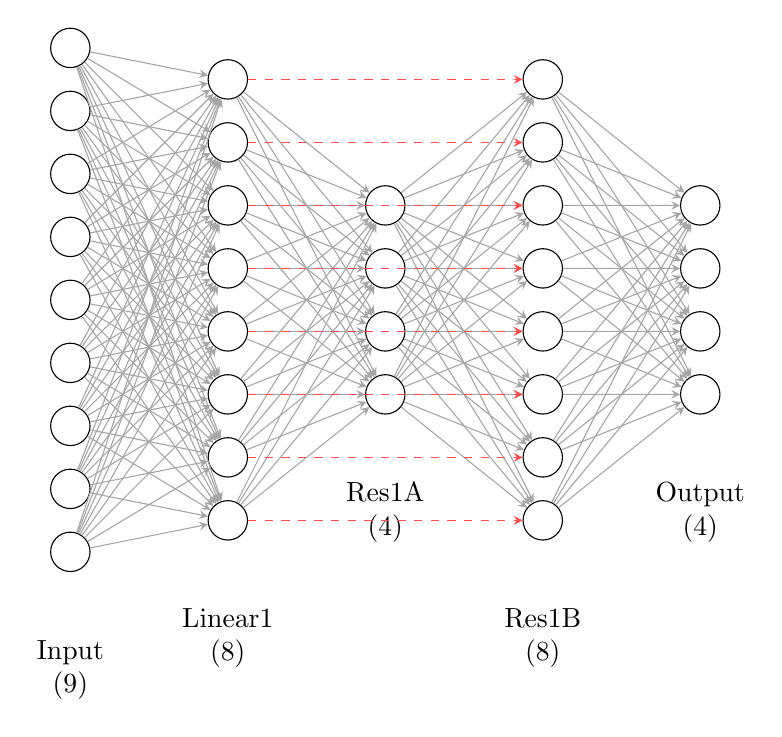
\begin{tikzpicture}[
        neuron/.style={circle, draw=black, minimum size=5mm, inner sep=0},
        >=stealth,
        node distance=1.5cm
    ]
        % 定义层参数:名称/数量/x位置
        \def\layers{
            Input/9/0, 
            Linear1/8/2, 
            Res1A/4/4, 
            Res1B/8/6,
            Output/4/8
        }

        % 绘制神经元
        \foreach \layername/\layercount/\x in \layers {
            \foreach \i in {1,...,\layercount} {
                \node[neuron] (\layername-\i) at (\x, {\i*0.8 - \layercount*0.4 - 0.4}) {};
            }
            \node[anchor=north, align=center] at (\x, {-\layercount*0.4 - 0.6}) {\layername\\(\layercount)};
        }

        % Input → Linear1
        \foreach \i in {1,...,9}{
            \foreach \j in {1,...,8}{
                \draw[->, gray!70] (Input-\i) -- (Linear1-\j);
            }
        }

        % Linear1 → Res1A
        \foreach \i in {1,...,8}{
            \foreach \j in {1,...,4}{
                \draw[->, gray!70] (Linear1-\i) -- (Res1A-\j);
            }
        }

        % Res1A → Res1B
        \foreach \i in {1,...,4}{
            \foreach \j in {1,...,8}{
                \draw[->, gray!70] (Res1A-\i) -- (Res1B-\j);
            }
        }

        % 残差连接(Linear1 → Res1B):虚线
        \foreach \i in {1,...,8}{
            \draw[->, dashed, red!70] (Linear1-\i) -- (Res1B-\i);
        }

        % Res1B → Output
        \foreach \i in {1,...,8}{
            \foreach \j in {1,...,4}{
                \draw[->, gray!70] (Res1B-\i) -- (Output-\j);
            }
        }

    \end{tikzpicture}	
    \caption{SmallResNet 网络结构(含残差连接)}
    \label{fig:SmallResNet}
\end{figure}


另一方面,我们还实现了一个小型的残差网络(smallResNet)如图\ref{fig:SmallResNet}所示,以期能取得更好的效果。该网络大体结构与smallMLP相同,但对于残差连接结构,使用了$8\rightarrow4\rightarrow8$的结构。Linear1层的输出结果,会直接与Res1A层的输出结果相加,作为Res1B层的输入,即图\ref{fig:SmallResNet}中的红色虚线所示。在这个网络中,共计使用\textbf{192}个参数。

\subsection{性能评估}

使用多层感知机与残差网络对数据集进行训练,得到如表\ref{tab:Classic Model Training Results}所示的实验结果。

\begin{table}[H]
\centering
\caption{经典模型的训练结果}
\label{tab:Classic Model Training Results}
\begin{tabular}{ccccc}
    \toprule
    \textbf{迭代次数} & \textbf{经典模型} & \textbf{训练准确率} & \textbf{测试准确率} & \textbf{测试F1分数} \\
    \midrule
    \multirow{2}{*}{50} & SmallMLP & 69.55\% & 66.10\% & 0.3993 \\
        & SmallResNet & 74.37\% & 75.30\% & 0.5564 \\
    \midrule
    \multirow{2}{*}{250} & SmallMLP & 86.98\% & 85.60\% & 0.6645 \\
        & SmallResNet & 87.02\% & 85.50\% & 0.6632 \\
    \midrule
    \multirow{2}{*}{500} & SmallMLP & 87.15\% & 85.50\% & 0.6635 \\
        & SmallResNet & 87.37\% & 85.80\% & 0.6662 \\
    \bottomrule
\end{tabular}
\end{table}

根据实验结果可知,在固定参数大小下,经典的神经网络模型ResNet与MLP的实验精度基本一样,使用更复杂的ResNet模型对实验的结果精度并未产生较大提升。从模型理论上看,由于更复杂的模型(ResNet)在提出的时候往往是解决增加模型参数却不能极大提高准确率的问题,而在该任务中所用经典参数较少,并未达到MLP的模型性能极限,因此使用ResNet并未提升较大精度。

由以上实验分析,我们可以提出如下假设:在固定参数下,存在经典模型并未超出其性能极限,即在固定参数下更改模型并不能提升预测精度。在此假设下,我们希望存在某种模型能够在原有经典模型的基础上,能进一步较大提升模型的预测精度,从而减少模型的参数量,进而提高模型的计算效率。

%%%%%%%%%%%%%%%%%%%%%%%%%%%%%%%%%%%%%%%%%%%%%%%%%%%%%%%%%%%%%%%%%%%%%%%%%%%%%%%%%%%%%%%%%%%%%%%%%%%%%%%%%%%%%%%%%%%%%%%%%%%%%%%

\section{量子机器学习模型}

\subsection{算法原理}

在本次报告中,我们实现的量子机器学习模型为QMLP(Quantum Multi-Layer Perceptron)。QMLP是基于变分量子算法的量子神经网络模型,主要由以下几个部分组成:

\subsubsection{量子数据编码}

QMLP采用线性旋转编码将经典数据映射到量子态:

\begin{equation}
S(\mathbf{x}) = \bigotimes_{k=1}^N RX(x_k) = \exp\left(-i\sum_{k=1}^N x_k \sigma_x^{(k)}/2\right)
\end{equation}
其中$\sigma_x^{(k)}$为第$k$个量子比特的Pauli-X算符。这个电路都构造非常简单,如图\ref{fig:Quantum Circuits}左图所示。

\begin{figure}[tb]
\centering
    \begin{quantikz}
        \lstick{$\ket{0}$} & \gate{RX(x_1)} & \\
        \lstick{$\ket{0}$} & \gate{RX(x_2)} & \\
        \lstick{$\vdots$} \wave&&& \\
        \lstick{$\ket{0}$} & \gate{RX(x_N)} &
    \end{quantikz}
    \qquad
    \begin{quantikz}
        \lstick{$\ket{\psi_1}$} & \ctrl{1} & \gate{RX(\theta_1)} & \\
        \lstick{$\ket{\psi_2}$} & \targ{}{} & \gate{RY(\theta_2)} &
    \end{quantikz}
\caption{左:量子数据编码电路;右:参数化纠缠层电路}
\label{fig:Quantum Circuits}
\end{figure}

\subsubsection{变分量子电路}

\begin{equation}
    U(\theta) = \prod_{l=1}^L U_l(\theta_l)R_l(\mathbf{x})
\end{equation}

其中:
\begin{itemize}
    \item $U_l(\theta_l)$:参数化量子门层
    \item $R_l(\mathbf{x})$:重上传单元
\end{itemize}

\subsubsection{动态非线性机制}

通过可调重上传单元(RUU)引入非线性:

\begin{equation}
    R_l(\mathbf{x}) = \exp\left(-i f_l(\mathbf{x}) \sigma_j^{(k)}/2\right), \quad j \in \{x,y,z\}
\end{equation}

典型配置包括:

\begin{itemize}
    \item $RX(\text{ReLU}(\mathbf{x}))$
    \item $RY(\mathbf{x}^2)$
    \item $RZ(\tanh(\mathbf{x}))$
\end{itemize}


\subsubsection{参数化纠缠层}

采用可训练的两比特门实现自适应纠缠,电路如图\ref{fig:Quantum Circuits}右图所示。

\begin{equation}
    CRX(\theta) = \begin{pmatrix}
    1 & 0 & 0 & 0 \\
    0 & 1 & 0 & 0 \\
    0 & 0 & \cos\theta/2 & -i\sin\theta/2 \\
    0 & 0 & -i\sin\theta/2 & \cos\theta/2 
    \end{pmatrix}
\end{equation}

\begin{algorithm}
    \caption{QMLP训练流程}
    \begin{algorithmic}[1]
    \State 初始化参数$\{\theta_l\}_{l=1}^L$和$\{f_l\}_{l=1}^L$
    \For{每个训练epoch}
        \State 编码输入:$\ket{\phi_0} = S(\mathbf{x})\ket{0}^{\otimes N}$
        \State 量子态演化:$\ket{\phi_L} = \prod_{l=1}^L U_l(\theta_l) R_l(f_l) \ket{\phi_0}$
        \State 测量期望值:$\langle Z\rangle_i = \bra{\phi_L} Z_i \ket{\phi_L}$
        \State 计算损失:$\mathcal{L} = -\sum_c y_c \log p_c$
        \State 通过参数偏移规则更新参数
    \EndFor
    \end{algorithmic}
\end{algorithm}

\begin{figure}[tb]
    \centering
    \smartdiagram[flow diagram:horizontal]{
        输入$\mathbf{x}$,
        线性编码,
        \shortstack{变分层1\\\footnotesize(RUU非线性)},
        参数化纠缠,
        \shortstack{变分层2\\\footnotesize(输出测量)}
    }
    \caption{QMLP算法流程图}
    \label{fig:qmlp_flow_smart}
\end{figure}

\subsection{实现细节}

出于效率的考量,我们采用了量子经典混合的架构,即首先由经典神经网络将9维的输入降维到4维,之后将这些数据输入到QMLP中,最后的测量结果就是输出。整个架构如图\ref{fig:QuantumMLP}之子图1所示,而其中的"Quantum Circuit"部分具体如图\ref{fig:QuantumMLP}之子图2所示。在子图2中,$Rot(\theta_{i}\sim\theta_{i+2})$表示了一套需要三个量子参数的$RX,RY,RZ$门组合,而四个相连受控位表示一套$CRX$门组合,需要四个量子参数,分别如图\ref{fig:QuantumMLP}之子图3,4所示。显而易见,在这个架构中,经典参数量为$9\times4+4=40$,而量子参数量为$8\times3+2\times4=32$个,总共\textbf{72}个参数。

\begin{figure}[tb]
\centering
    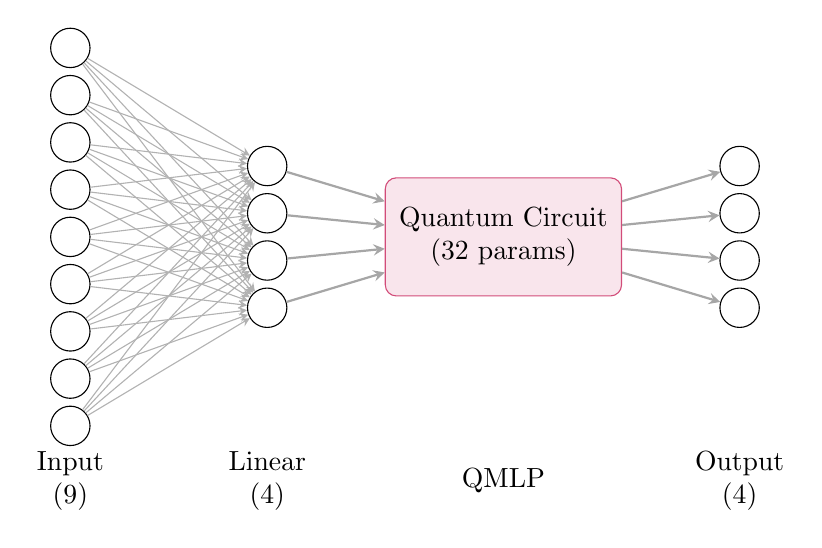
\begin{tikzpicture}[
        neuron/.style={circle, draw=black, minimum size=5mm, inner sep=0},
        quantum/.style={rectangle, draw=purple!70, fill=purple!10, minimum width=3cm, minimum height=1.5cm, rounded corners, align=center},
        >=stealth,
        every label/.style={text width=2cm, align=center}
    ]

        % 定义各层节点数及间距
        \def\inputN{9}
        \def\linearN{4}
        \def\outputN{4}
        \def\dy{0.6}  % 垂直间距

        % 计算最大层数以居中对齐
        \pgfmathsetmacro{\maxN}{max(\inputN,\linearN,\outputN)}
        \pgfmathsetmacro{\centerY}{(\maxN - 1) * \dy / 2}

        % Input layer
        \foreach \i in {1,...,\inputN} {
            \pgfmathsetmacro{\y}{(\i - 1) * \dy - (\inputN - 1) * \dy / 2}
            \node[neuron] (input-\i) at (0, \y) {};
        }
        \node[align=center] at (0, -\centerY - 0.7) {Input\\(\inputN)};

        % Linear layer
        \foreach \i in {1,...,\linearN} {
            \pgfmathsetmacro{\y}{(\i - 1) * \dy - (\linearN - 1) * \dy / 2}
            \node[neuron] (linear-\i) at (2.5, \y) {};
        }
        \node[align=center] at (2.5, -\centerY - 0.7) {Linear\\(\linearN)};

        % Quantum Circuit block(居中即可)
        \node[quantum] (quantum) at (5.5, 0) {Quantum Circuit\\(32 params)};
        \node at (5.5, -\centerY - 0.7) {QMLP};

        % Output layer
        \foreach \i in {1,...,\outputN} {
            \pgfmathsetmacro{\y}{(\i - 1) * \dy - (\outputN - 1) * \dy / 2}
            \node[neuron] (output-\i) at (8.5, \y) {};
        }
        \node[align=center] at (8.5, -\centerY - 0.7) {Output\\(\outputN)};

        % Input → Linear
        \foreach \i in {1,...,\inputN}{
            \foreach \j in {1,...,\linearN}{
                \draw[->, gray!60] (input-\i) -- (linear-\j);
            }
        }

        % Linear → Quantum
        \foreach \i in {1,...,\linearN}{
            \draw[->, thick, gray!70] (linear-\i) -- (quantum);
        }

        % Quantum → Output
        \foreach \i in {1,...,\outputN}{
            \draw[->, thick, gray!70] (quantum) -- (output-\i);
        }

    \end{tikzpicture} \\

    % \vspace{0.1cm}
    \noindent\makebox[\textwidth]{\dotfill}
    \vspace{0.01cm}

    \begin{quantikz}[row sep=0.3cm, column sep=0.5cm]
        \lstick{$q_0$} & \gate{R_x(x_0)} & \gate{Rot(\theta_0\sim\theta_2)} & \ctrl[vertical wire=c]{3} & \gate{R_x(x_0)} & \gate{Rot(\theta_{16}\sim\theta_{18})} & \ctrl[vertical wire=c]{3} & \meter{} \\
        \lstick{$q_1$} & \gate{R_x(x_1)} & \gate{Rot(\theta_3\sim\theta_5)} & \control{}   & \gate{R_x(x_1)} & \gate{Rot(\theta_{19}\sim\theta_{21})} & \control{}   & \meter{} \\
        \lstick{$q_2$} & \gate{R_x(x_2)} & \gate{Rot(\theta_6\sim\theta_8)} & \control{} & \gate{R_x(x_2)} & \gate{Rot(\theta_{22}\sim\theta_{24})} & \control{} & \meter{} \\
        \lstick{$q_3$} & \gate{R_x(x_3)} & \gate{Rot(\theta_9\sim\theta_{11})} & \control{}   & \gate{R_x(x_3)} & \gate{Rot(\theta_{25}\sim\theta_{27})} & \control{}   & \meter{} \\
    \end{quantikz} \\

    \noindent\makebox[\textwidth]{\dotfill}
    \vspace{0.01cm}

    \begin{quantikz}
        & \gate{Rot((\theta_{i}\sim\theta_{i+2}))} & 
    \end{quantikz} \quad=\quad \begin{quantikz}[column sep=0.1cm]
        & \gate{RX(\theta_{i})} & \gate{RY(\theta_{i+1})} & \gate{RZ(\theta_{i+2})} & 
    \end{quantikz} \\

    \noindent\makebox[\textwidth]{\dotfill}
    \vspace{0.01cm}

    \begin{quantikz}
        & \ctrl[vertical wire=c]{3} & \\ & \control{} & \\ & \control{} & \\ & \control{} &
    \end{quantikz} \quad=\quad \begin{quantikz}[row sep=0.04cm, column sep=0.05cm]
        & \ctrl{1} & & & \gate{RX(\theta_{i+3})} &\\
        & \gate{RX(\theta_{i})} & \ctrl{1} & & & \\
        & & \gate{RX(\theta_{i+1})} & \ctrl{1} & & \\
        & & & \gate{RX(\theta_{i+2})} & \ctrl{-3} &
    \end{quantikz}

\caption{\centering 自上而下:子图1:QuantumMLP 网络结构图:线性映射 + 参数化量子电路 + 测量输出;\\ 子图2:参数化量子电路的具体实现;\\ 子图3:$Rot(\theta_{i}\sim\theta_{i+2})$门的具体实现;\\ 子图4:$CRX$门组合的具体实现。}
\label{fig:QuantumMLP}
\end{figure}

% \begin{quantikz}[row sep=0.5cm, column sep=0.5cm]
%     \lstick{$q_0$} & \gate{R_x(x_0)} & \gate{Rot(\theta_0)} & \ctrl{1} & \gate{R_x(x_0)} & \gate{Rot(\theta_1)} & \ctrl{1} & \meter{} \\
%     \lstick{$q_1$} & \gate{R_x(x_1)} & \gate{Rot(\theta_3)} & \targ{} & \gate{R_x(x_1)} & \gate{Rot(\theta_4)} & \targ{} & \meter{} \\
%     \lstick{$q_2$} & \gate{R_x(x_2)} & \gate{Rot(\theta_6)} & \ctrl{1} & \gate{R_x(x_2)} & \gate{Rot(\theta_7)} & \ctrl{1} & \meter{} \\
%     \lstick{$q_3$} & \gate{R_x(x_3)} & \gate{Rot(\theta_9)} & \targ{} & \gate{R_x(x_3)} & \gate{Rot(\theta_{10})} & \targ{} & \meter{}
% \end{quantikz}


\subsection{性能评估}

%%%%%%%%%%%%%%%%%%%%%%%%%%%%%%%%%%%%%%%%%%%%%%%%%%%%%%%%%%%%%%%%%%%%%%%%%%%%%%%%%%%%%%%%%%%%%%%%%%%%%%%%%%%%%%%%%%%%%%%%%%%%%%%

\section{性能对比与分析}

\subsection{性能对比}

\begin{table}[H]
    \centering
    \caption{经典机器学习与量子机器学习的性能对比}
    \label{tab:Performance Comparison of Classical and Quantum Models}
    \begin{tabular}{ccccc}
        \toprule
        \textbf{模型} & \textbf{参数量} & \textbf{训练准确率} & \textbf{测试准确率} & \textbf{测试F1分数} \\
        \midrule
        经典小型ResNet & 192 & 87.37\% & 85.80\% & 0.6662 \\
        量子经典混合MLP & 72 & \% & \% & 0. \\
        \bottomrule
    \end{tabular}
\end{table}
    

\subsection{差异分析}



%插入表格(三线表)
% \begin{table}[htbp]
%     \centering
%     \caption{表题}
%     \begin{tabular}{ccccc}%{{5}{c}}

%         \toprule
%         {组别} & {物理量1/单位} & {物理量2/单位} & {物理量3/单位} & {物理量4/单位} \\
%         \midrule
%         A&{}&{}&{}&{}\\
%         B&{}&{}&{}&{}\\
%         C&{}&{}&{}&{}\\
%         D&{}&{}&{}&{}\\
%         \bottomrule
%     \end{tabular}
% \end{table}


%插入图片
% \begin{figure}[htbp]
%     \centering 
%     \includegraphics[height=5.99cm,width=8.25cm]{E:/engineer file/latex/learn1/photo/test.png}
%     \caption{图注}
% \end{figure}
%table和figure为浮动体






%%%%%列出参考文献%%%%%
\zihao{-5}%设置参考文献字号
\bibliography{books}%调用bib文件 加入参考文献
%知网复制出的latex代码比工大图书馆复制出的latex代码好用

%%%%%%%%%%%%%%%附录部分%%%%%%%%%%%%%%%
% \newpage
% \appendix%设置附录
% \zihao{-5}%设置附录字号
% \section*{附录一:}




\end{document}